\chapter{RFP Equilibrium}

\section{Magnetic confined plasma experiments}

Among the several proposed solutions for thermonuclear confinements devices, the torus appeared as the most topological advantageous: the torus, indeed, is the only compact manifold connected and orientable where it is possible to define a continuous vector field without critical points\footnote{that is: once a vector field has been defined on the surface of the torus, there are any point where it goes to zero; this characteristic let the field lines to reconnect on themselves minimizing the energy spent and maximizing the stability of the plasma}.
In this case the field configurations consist on a set of magnetic toroidal and poloidal components. In \Figure{\ref{fig:intro_toroidal_coords}} a toroidal coordinates ($r,\theta,\varphi$) reference system is represented, where:
\begin{figure}[h!]
    \centering
    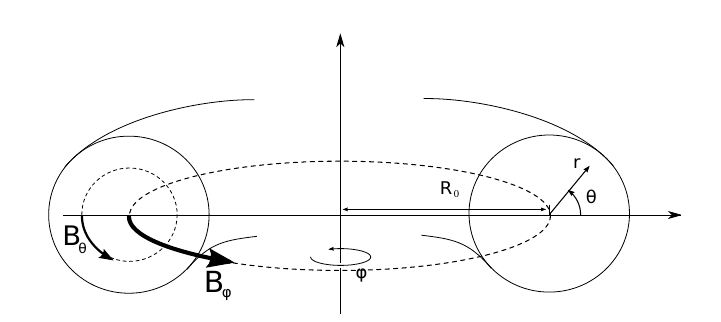
\includegraphics[width=8cm]{img/1_intro/toroidal_coords.png}
    \caption{Toroidal coordinates reference system}
    \label{fig:intro_toroidal_coords}
\end{figure}
\begin{itemize}
    \item $r = $ radial distance from central circular axis,
    \item $\vartheta = $ poloidal angle,
    \item $\varphi = $ toroidal angle.
\end{itemize}
Depending on their characteristics, the magnetic confined machines are divided in three principal categories:
\begin{itemize}
    \item \textit{Tokamak}, where both the toroidal field and poloidal field components are present but with a net toroidal predominance that assumes essentially stabilization functions.
    \item \textit{RFP}, where the toroidal component is almost comparable to the poloidal to the extent that it reaches an inverted value at the boundary ( hence the name "\textit{reversed} field pinch"). Compared to the Tokamak configuration here the stability of plasma is much more critical, but with higher efficiency.
    \item \textit{Stellarator}, where the geometry of the field is built by a complex displacement of non planar coils that encourage the winding of the plasma column.
\end{itemize}

\subsubsection{Tokamak configuration}
In the \textit{Tokamak} systems the toroidal field $B_\varphi$ is produced by a toroidal solenoid winded around the vacuum chamber, while the poloidal field $B_\vartheta$ is created by a strong toroidal current $I_p$ that flaws within the plasma. This current is in turn induced by means of solenoids coupled by the plasma ring (sometimes concatenated with a central coil). The same current is also used to heat the plasma by Joule effect ( Ohmic heating ) with a specific power of $P = \eta J^2$, defined $\eta$ as the plasma resistivity.
%
A fundamental parameter to define the \textit{Tokamak} typical features is $\beta$ defined as:
\begin{equation}
    \beta = \frac{<p>}{ \frac{B(a)^2}{2\mu_0} }
    \label{eq:magnetic_beta}
\end{equation}
with $<p>$ the average value of plasma pressure within a poloidal section. This parameter is the ratio between the mean kinetic pressure exerted by plasma, and the magnetic pressure of the field that is needed to confine it; the value assumed by $\beta$ is thus the measure of how effective the magnetic configuration results when seen as an energy balance.
If we compute the \eqref{eq:magnetic_beta} using the typical $B_\varphi$ and $B_\vartheta$ values that are present in a \textit{tokamak}, the resulting $\beta$ is about $2~3\%$; this means that the most of the spent energy that \textit{Tokamak} uses is not for the confinement but is is almost all used to stabilize perturbations.
Another key factor that defines the relative intensities of magnetic configuration is the so called "\textit{safety factor}" $q$:
\begin{equation}
    q(r) = \frac{rB_\varphi(r)}{R_0B_\vartheta(r)}
\end{equation}
As it will be widely described in the following sections, the radial profile of this parameter has a fundamental impact on the overall stability of the plasma: it more detail a stable plasma configuration can be obtained by maintaining the $q(r)$ function strictly monotonic.
\begin{figure}
    \centering
    \subfigure[]{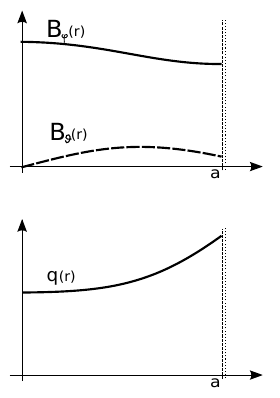
\includegraphics[height=5cm]{img/1_intro/tokamak_profiles.png} \label{fig:intro_safety_factor_profiles_a}}
    \subfigure[]{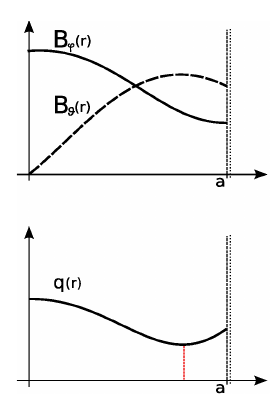
\includegraphics[height=5cm]{img/1_intro/rfp_profiles_norev.png} \label{fig:intro_safety_factor_profiles_b}}
    \subfigure[]{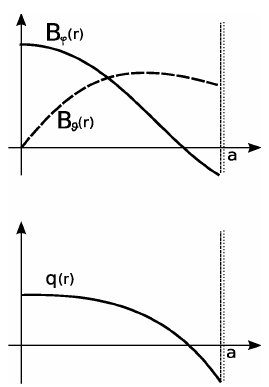
\includegraphics[height=5cm]{img/1_intro/rfp_profiles_rev.png} \label{fig:intro_safety_factor_profiles_c}}
    \caption{Magnetic field profiles for $B_\varphi$ and $B_\vartheta$, from the toroidal axis to the chamber boundary, for the toroidal confinement devices in \textit{Tokamak} configuration (a), \textit{RFP} without reversal (b), and \textit{RFP} with reversal (c)    }
    \label{fig:intro_safety_factor_profiles}
\end{figure}
As shown in \Figure{\ref{fig:intro_safety_factor_profiles_a}}, the the case of the \textit{Tokamak} configuration the monotonic property of the safety factor is guaranteed by an high ratio of $B_\varphi/B_\vartheta$. Although, because the poloidal fields is generated by the plasma current, to have such a high ratio of the fields it is necessary to maintain it under a certain threshold. This condition implies a in effects a limitation for the possible Ohmic heating bringing with it the need to find other means of additional heating: neutral particles injections (NBI), radio-frequency emission resonating with cyclotron frequencies of electrons or ions, etc.

\subsubsection{RFX configuration}
The \ac{RFP} is an axial-symmetric configuration provided with a toroidal current, similar to what has been presented for \textit{Tokamak}. The difference between the former and the latter case is in the ratio between the components of the magnetic field: while for \textit{Tokamak} the toroidal field is of one order of magnitude over the poloidal, for the \textit{RFP} the two components are almost the same in average, and in the outer region the poloidal one tends to dominate. As a result, the most part of the magnetic field is generated from the plasma current itself, and with the same plasma current the total magnetic field that is exploited by \acs{RFP} is much lower that the one used by a \textit{Tokmak}. It can be also seen that, in the right conditions, once the plasma current has been induced the toroidal field at the boundary inverts direction; this reversal gives a chance to obtain a monotonic factor $q(r)$ even with a this low magnetic profiles. This is generally facilitated inverting the current direction on the coils of the toroidal system some instants after the pulse begins. For the \acs{RFP} model the profiles of $B_\varphi$(r), $B_\vartheta(r)$ and $q(r)$ are reported in \Figure{\ref{fig:intro_safety_factor_profiles_b}} and \Figure{\ref{fig:intro_safety_factor_profiles_c}} in the pre-reversal and reversal conditions.

Together with this reduced toroidal field intensity comes the possibility of reaching $\beta$ values much higher than the ones that characterize the \textit{Tokamak}. Although the high penalty payed by the \textit{RPF} is in the stability of perturbations that represents a profound limitation for the final achievable temperature, that remains one order of magnitude lower that the one promised by \textit{Tokamak}.
 

% 
In the Tokamak configuration and the Reversed Field Pinches (RFPs), because the magnetic field is generated by both external coils and the plasma current  belongs to pinch family. 
%
The toroidal field in tokamaks is generated by external coils and the poloidal component is generated by the plasma current, which is induced by the primary transform. In advanced tokamak scenario, however, most of the poloidal field component is generated by the so-called ’bootstrap’ current which is induced by the density gradient. Nevertheless, the disadvantage for tokamak configuration is that it suffers a limitation of plasma current due to plasma instability. Consequently, extra heating method besides Ohmic heating is needed for plasma fusion in tokamaks. 
%
% \begin{figure}[ht!]
% 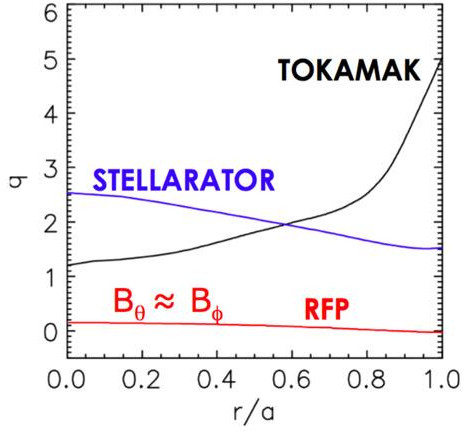
\includegraphics[width=0.5\textwidth]{img/safety-fact.jpg} \centering
% \caption{Generic safety factor profiles for the tree main devices configurations (Tokamak, RFP, Stellarator).}
% \label{rfx}
% \end{figure}
%

% RW
The RFP is a toroidal configuration for the magnetic confinement of thermonuclear plasmas. The RFP shares with the tokamak similar features, for example the presence of two components of the confining magnetic field: a toroidal component $B_t$ and a poloidal one, $B_p$ , and the pinch effect. The latter means that a toroidal electric current is driven in a plasma, which is embedded in a toroidal magnetic field. Different from the tokamak, the applied toroidal magnetic field is extremely small. The plasma toroidal magnetic field, which is of the same order of magnitude as the poloidal field another significant difference with respect to the tokamak where the toroidal magnetic field is one order of magnitude larger than the poloidal is mainly produced by electrical currents flowing in the plasma through a self-organization process and changes sign at the plasma edge with respect to the core. Given its magnetic topology, the RFP exploits the advantage of an easier technology involved in the electromagnetic system. This might be the case even for a reactor, where there might be no need for large superconducting magnetic coils; there is freedom in the choice of the aspect ratio and in principle ignition should be achievable with ohmic heating only. 
% RW
A price to be paid for exploiting these advantages concerns magneto-hydrodynamic (MHD) stability. The safety factor q is in fact lower than 1 across the whole plasma, and negative at the edge. Figure 2(a) shows the q profiles of an RFP compared with those of tokamaks and stellarators. In the RFP q profile there are multiple resonant surfaces in the plasma, in particular for modes with poloidal mode numbers m = 0 and 1. This is shown in figure 2(b), which reports a typical RFP q profile. Two main kinds of global, current-driven MHD instabilities may be present in a RFP with resistive wall: (i) resistive kink/TMs, which are resonant in the plasma and are intrinsically linked to the sustainment of the configuration through the aforementioned self-organization process. (ii) RWMs, which are non-resonant ideal modes, slowed down by the resistive wall. RWMs in RFP are current driven and are present also at low plasma beta.


RFPs, however, can sustain very high plasma current and this makes it to be considered a potential fusion device with only Ohmic heating. On the other hand, the generation of plasma current needs a time variation of magnetic field which is sustained by the primary transform. This time variation makes the devices, on some level, not in steady state. To overcome this problem, a toroidal configuration which all the field components are generated by external coils is introduced. This device is the so-called stellarators. Figure 1.3 shows a sketch of these two families. In the left graph, the red coils aligned toroidally are the toroidal field coils and the green helical ones are helical field coils. In the right graph, the red cylinder in the device center is the primary transformer. The red coils aligned toroidally are the toroidal field coils and the two green ones in the top and bottom of the device is the vertical stabilization coils. The stabilization coils are introduced because due to the existence of Shafranov shift in toroidal devices, the plasma position needs to be optimized in order to avoid touches between magnetic field and the first wall. 
The stellarator shows a much more complicated magnetic coil design than one in pinch family. Consequently, the manufacture process for magnetic coils are more complex for stellarators than for pinches. On the other hand, due to lack of plasma current in stellarators, it is almost free of disruptions.


%% STELLARATOR HEATING ~ CURRENT
Unlike the z-pinch designs being explored in the UK and other US labs, the stellarator has no induced electrical current within the plasma - at a macroscopic level, the plasma is neutral and unmoving, in spite of the individual particles within it rapidly circulating. In pinch machines, and the later tokamaks, the current itself is one of the primary methods of heating the plasma. In the stellarator, no such natural heating source is present.

Early stellarator designs used a system similar to those in the pinch devices to provide the initial heating to bring the gas to plasma temperatures. This consisted of a single set of windings from a transformer, with the plasma itself forming the secondary set. When energized with a pulse of current, the particles in the region are rapidly energized and begin to move. This brings additional gas into the region, quickly ionizing the entire mass of gas. This concept was referred to as ohmic heating because it relied on the resistance of the gas to create heat, in a fashion not unlike a conventional resistance heater. As the temperature of the gas increases, the conductivity of the plasma improves. This makes the ohmic heating process less and less effective, and this system is limited to temperatures of about 1 million kelvins.[36]

%% RFP
% - Taylor relaxed state (need of reversal) -> magnetic shear
% - reversal can not be produced by coils ... plasma is needed
% - no need for superconducting coils and no current limit  -we don't satisfy Kruskal-Shafranov (safety factor)-
%   (10MA target to have a good condition in terms of neutrons production) -> ohmic heating is possible.
% - In RFX-mod the ohmic heating power can scale up to 60MW of coupled power (that is a huge amount of power)
%   in a stellarator to reach the same power deposition using external heating you need very high power.
% - High current possibility means -> High particle density limit ... Greenwald limit

% - why High plasma current? because 

\section{MHD, Fourier analysis, equilibrium and Modes control}
% There are several techniques to represent magnetic confinement (orbits - MHD) (brief)
% MHD is the best description to macroscopically describe the plasma as a fluid
% MHD - ideal (single double fluid)
% MHD - resistive (brief)
% Instabilities

\section{RFX-mod2 \\ \small{the opportunity of the best controllable machine}}
\cite{SONATO2003161}
\cite{doi:10.1063/1.4806765}
\cite{martin_RFX_overview}

% CHALLENGES AND SOLUTIONS IN THE DESIGN OF RFX-MOD2, A MULTI CONFIGURATION MAGNETIC CONFINEMENT EXPERIMENTAL DEVICE


% RWR
RFX-mod is a flexible \ac{RFP} toroidal device (major radius $R=2 m$ and minor radius $a=0.46 m$) with plasma current up to 2 MA \cite{2MA_RFX_Current} and volume $10 m^3$ \cite{SONATO200597}. As in all RFPs, plasma heating is purely ohmic; \acl{RFP} could in principle obtain fusion power with ohmic heating only, and with magnetic field much smaller than in a tokamak—avoiding superconducting coils. RFX-mod is equipped with a very powerful system of active coils for feedback control of plasma MHD stability: 192 coils, independently driven, cover the whole plasma surface.
% RWR
The major challenges of RFP research, and of RFX-mod in particular, are (a) rapidly advancing its performance, to assess the viability of the RFP approach to fusion; (b) providing a state-of-the-art contribution to the global task of feedback control of MHD stability, with experiments done both in RFP and in tokamak configuration; (c) focusing on the key topic of 3D magnetic shaping in a growing collaboration with the stellarator community; (d) training a new generation of fusion scientists.



\begin{figure}[ht!]
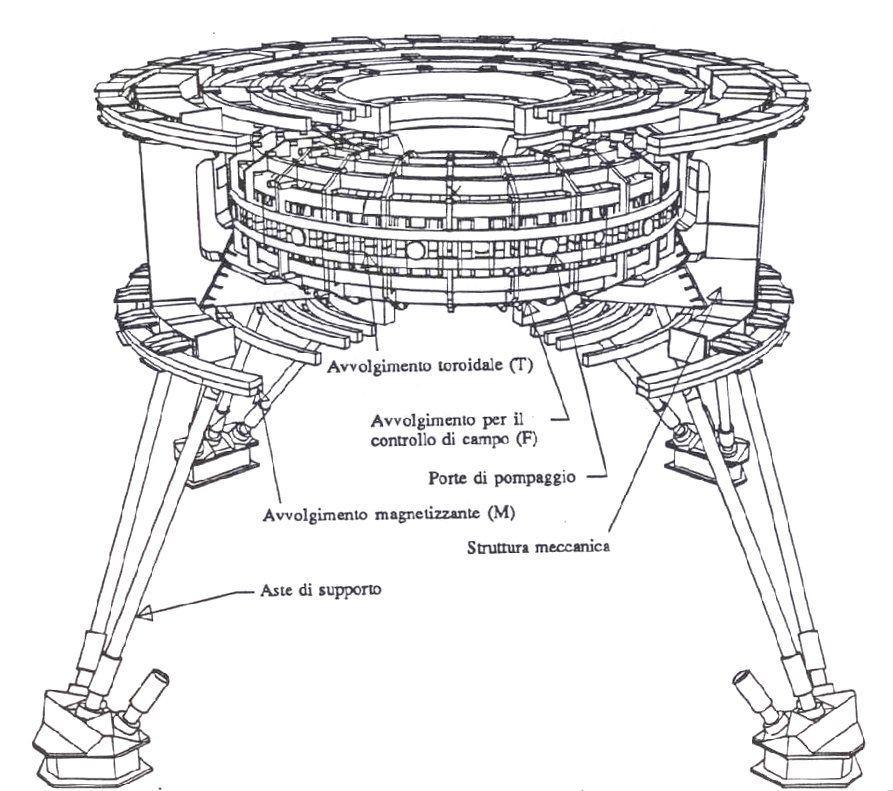
\includegraphics[width=0.5\textwidth]{img/rfx2}
\centering
\caption{RFX-mod sketch}
\label{rfx}
\end{figure}

\section{RFX diagnostics}
% kind of RFX diagnostics

%
\begin{figure}[ht!]
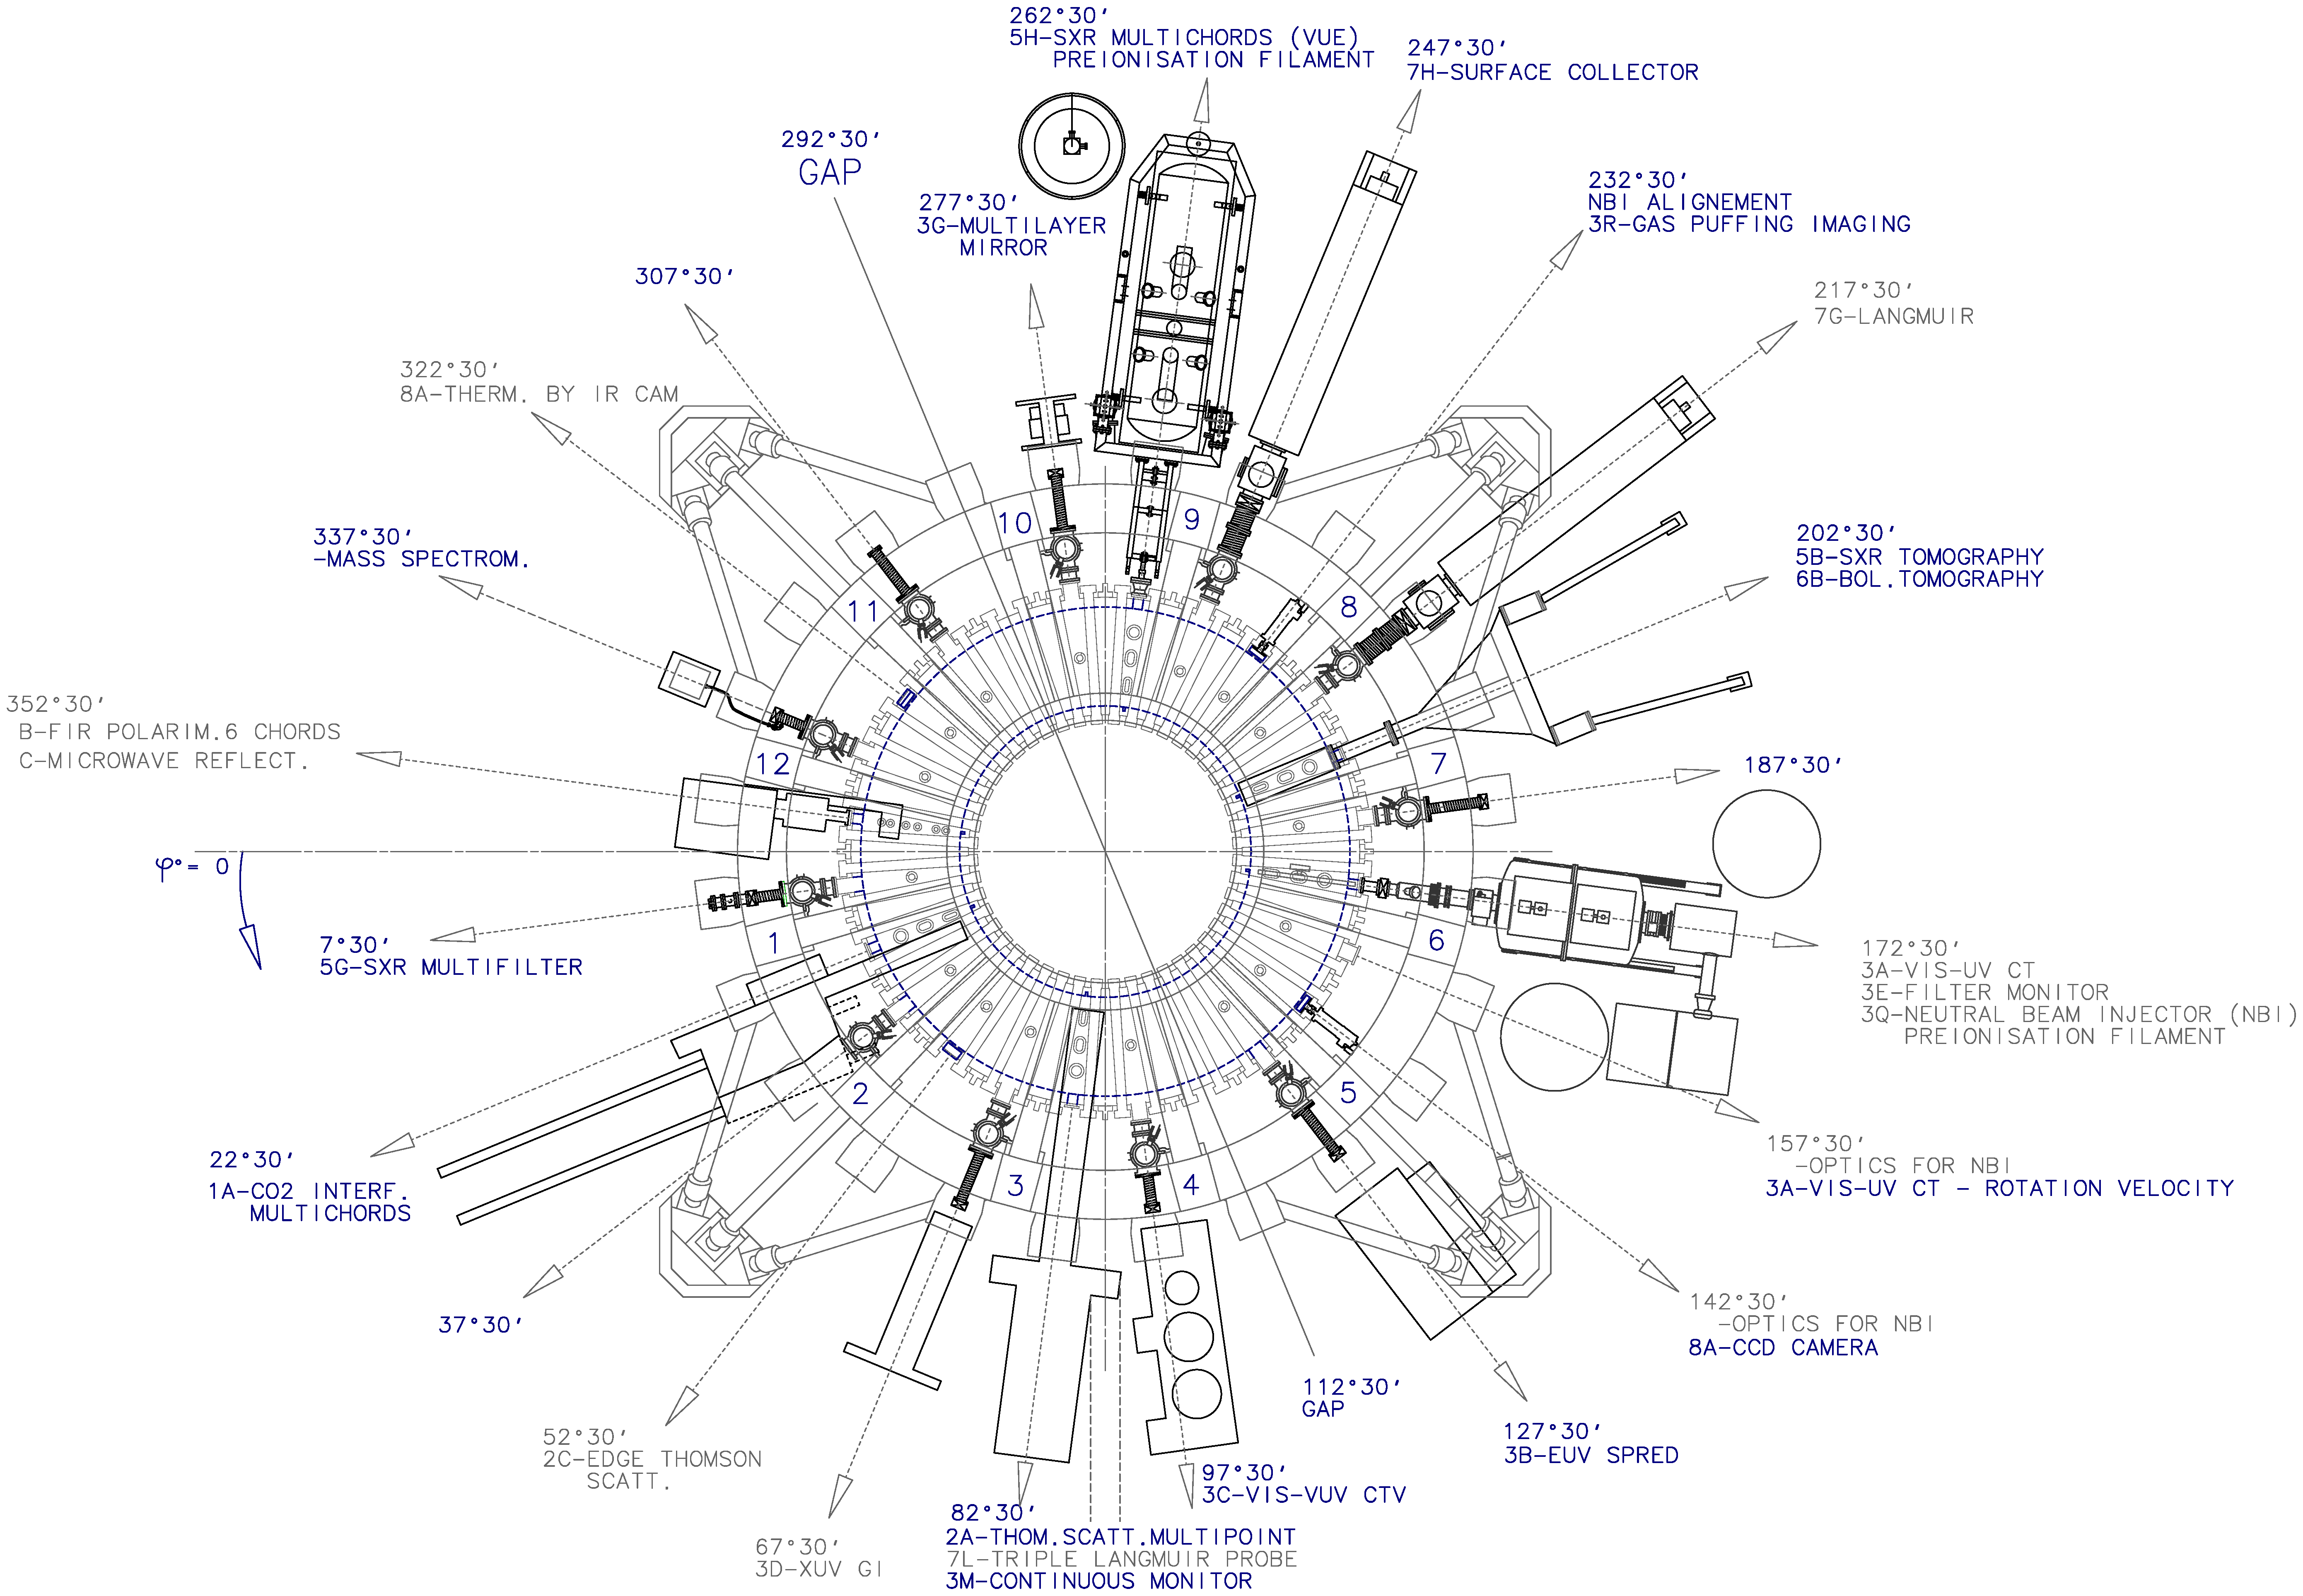
\includegraphics[width=1\textwidth]{img/rfx/Layout_Diagnosiche_AA10005.eps} \centering
% TODO: add figures
\caption{RFX map of diagnostics with related toroidal position.}
\label{rfx}
\end{figure}
%

\subsection{Thomson Scattering}
The Thomson scattering  has been a key-factor diagnostic at RFX since the initial operations for the study of RFP plasma configuration, yielding a fundamental correlation between the electron temperature diffusivity and the magnetic fluctuations that link the plasma confinement to the dynamo related modes~\cite{}. This also evolved in the possibility to identify a hot asymmetric island when the temperature gradient extends to the plasma core in the \ac{QSH} state.
During the first operation of RFX the diagnostic was composed by a single pulse of laser from ruby diode ( $\lambda = 694 nm$ ) passing through the plasma in the equatorial plane, and two grating photomultipliers spectrometers.
This apparatus presented some limitations: from the precision point of view it suffered of a poor quantum efficiency of the multialkali photocathode of the photomultiplier (MCP-PMT) resulting in a general lack of sensitivity and noisy profile at low electron temperatures. On the other hand the 20 chords acquisition that characterized the acquired plrofile with a 24 mm spatial resolution was unable to effectively investigate the details of the QSH magnetic islands.

Since the 2005 with the experiment upgrade to RFX-mod the diagnostic was completely renewed. In particular the replacement of the grating spectrometers with a set of four filter polycromators with avalance photodiodes (APD) provided a 30 times higher sensitivity and 84 points profile with a new narrow grained 7mm resolution ( $r/a$ from -0.96 to 0.84 ).
The new Nd:YLF laser diode ($\lambda=1053 nm$) located 15 m away from the center of the vacuum vessel, can produce an up to 7 J burst of 10 pulses per experiment shot. with a single light emission duration of 20ns $\ac{FWHM}$.

The light passing through plasma on the equatorial plane scatter in all directions and is collected by photomultipliers at three different windows at the end of short vertical ports. The 84 pairs of quarz fibers look all the plasma poloidal angles seen by magnifying optics located at the ports. All fibers can be also moved by a special mechanical support that can self orient during the experiment setup state; at the same time all optics can also automatically adjust focus to the desired radial position of interest.
A further side by side light path decomposes the acquired spectrum in 4 channels using a series of relay lenses.

The small amount of the solid angle covered by the acquisition, together with all this set of filters applied both at the input beam - aiming at reducing the stray light and maintaining the focus -, and at the output - for the selection of the plasma region of interest and for the decomposition of the energy spectrum - are the main reason for the required high power input.

This leads to a scattered set of acquisition pulses that are not continuously reconstructing the overall shape of plasma temperature but reduce ti a small set of usually 10 time events.

The recording systems is also quite complex: for RFX-mod the detected signal has been acquired by a modular 4-channels cPCI board dedicated for each of the spectrometers, acquiring data at 500 Msps each.

\subsection{Soft X Ray}

% We chose the most reliable and fast response diagnostics ... (SXR and Magnetic coils MHD)
% Other possible diagnostics can be added ( cope with time dim )
% Possibility to trigger in realtime other diagnostics ( i.e. Thomson Scattering )

\section{MHD}

\section{Newcomb SH}

\section{The complete “SCHEMA” from sensors to plasma parameters}
